\chapter{系统测试}
\thispagestyle{fancy}

\section{红外图像候选区域提取实验结果}


本系统采用两路视频源进行图像处理,包含红外图像处理以及光学图像处理。为了得到正确的候选区域坐标,需要求解两个相机坐标系之间的转换关系,如图\ref{红外与光学相机坐标系之间关系}所示。
\begin{figure}[h]
    \centering
    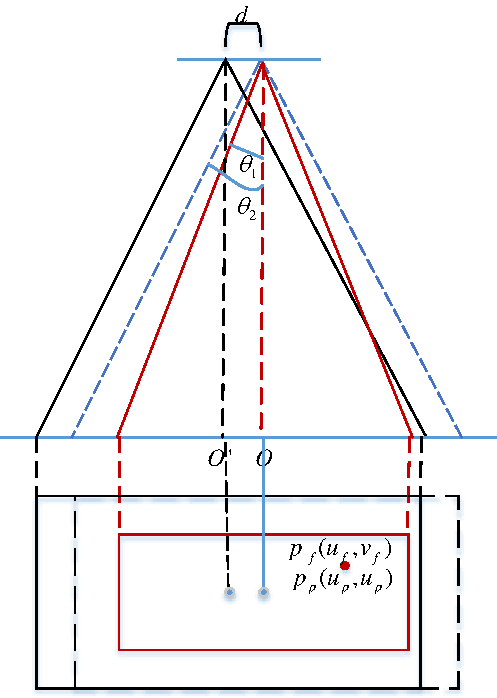
\includegraphics[height=7cm]{figures/红外与光学相机坐标系之间关系.pdf}
    \caption{红外与光学相机坐标系之间关系}\label{红外与光学相机坐标系之间关系}
\end{figure}

$\theta_1$为红外热像仪的视场角,$\theta_2$为光学相机的视场角大小(以$x$轴为例),$d$为两个成像系统轴心点的位置差。则红外相机图像坐标系中的点$p_f(u_f,v_f)$将通过下列变换映射到光学相机的图像坐标$p_p(u_p,v_p)$。先考虑共轴时(蓝色虚线与红色实线)的情况,有以下关系:	
\begin{gather}
u_p=u_{p0}+Width_P\cdot(u_f-u_{f0})/Width_F\\
v_p=v_{p0}+Height_P\cdot(v_f-v_{f0})/Height_F
\end{gather}
式中,$Width_P(Width_F)$和$Height_P(Height_F)$分别为光学(红外)图像的宽度和高度。实际上两个相机成像系统不共轴,安装位置有一个水平的偏差$d$,此时上式中的$u_p$变为:

\begin{equation}
u_p=u_{p0}+Width_P\cdot(u_f-u_{f0})/Width_F+d/fx
\end{equation}

$v_p$不变。其中$fx$是光学相机成像系统中每个像素代表的实际物理尺寸长度,在飞行高度很大的时候,$d/fx$是一个很小的数值,由于红外图像处理的结果是提取目标候选区域,因此也可以忽略该项。此外,系统使用的光学相机畸变很小,不加考虑。

根据第三章介绍的方法,机载计算设备通过AV视频采集卡,获取热成像视频数据,并进行处理,处理的结果为一系列坐标位置,代表目标候选区域。同时将红外图像进行伪彩化处理,输出到二进一出视频选择器,以供地面指令切换回传红外视频:计算设备接收飞机推送的切换指令之后,经由USB红外遥控功能令切换器进行视频源切换,再将视频通过高清图传传回地面。红外视频回传到地面站对于本系统扩展到夜间救援提供了可能。天空端的坐标回传和指令接收是通过DJI Onboard SDK数据透传功能实现。数据处理流程框图如图\ref{红外视频处理框图}所示。

\begin{figure}[h]
    \centering
    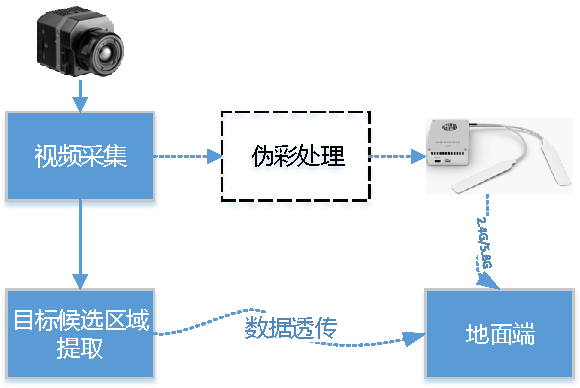
\includegraphics[height=5.5cm]{figures/红外视频处理框图.pdf}
    \caption{红外视频处理框图}\label{红外视频处理框图}
\end{figure}

由第三章介绍的处理算法,得到红外图像目标候选区域提取效果如图\ref{BoundingBoxResult}所示。
 	 
\begin{figure}[h]
    \centering
    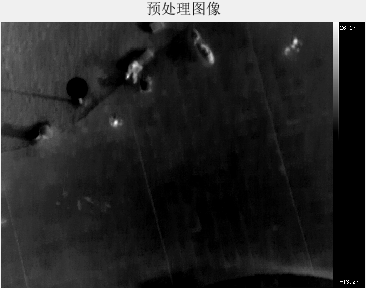
\includegraphics[height=3.5cm]{figures/红外目标候选区域提取结果1.png}
    \quad
    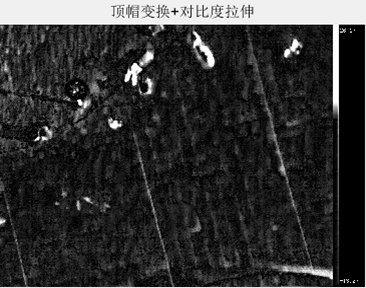
\includegraphics[height=3.5cm]{figures/红外目标候选区域提取结果2.png}
    
    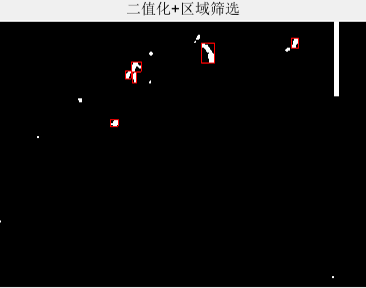
\includegraphics[height=3.5cm]{figures/红外目标候选区域提取结果3.png}
    \quad
    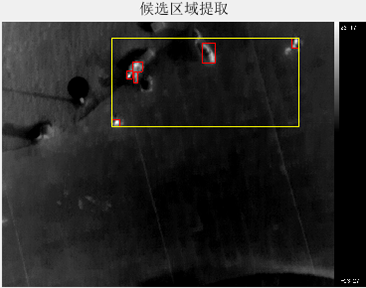
\includegraphics[height=3.5cm]{figures/红外目标候选区域提取结果4.png}
    \caption{红外目标候选区域提取结果}\label{BoundingBoxResult}
\end{figure}

考虑到实际搜救场景,搜救目标不会分布太分散。因此,在处理红外图像得到所有目标候选区域框之后,计算它们的最小外接矩形框,将此矩形的四个顶点坐标回传,即上图中黄色矩形框的四个顶点。

地面端根据两个成像系统之间的图像坐标转换关系,得到目标候选区域在光学图像上的对应位置,将其设为光学图像的ROI(Region Of Interest),并基于此ROI进行光学目标检测。这样一来,可以大大减少不必要的计算,进一步提高目标检测的性能。因为使用原图1080P大小进行处理,势必会增加计算时间。使用红外检测结果设置的ROI不仅可以提高搜索效率,还可以方便地面工作人员进行观察。




\section{光学目标检测结果}

为了便于对改进后的SSD算法进行训练,建立了自己的无人机视角下人体数据集,目前,数据集只标注了“人”(person)这一类,仿照了著名的行人数据库INRIAPerson (2416个训练正样本,$90\times160$大小),包含目标的训练图片为2680张,大小为 $1280\times720$(720P)。其中每一张中至少包含一个 ($1\sim10$) 目标样本,每个正样本都有对应的Ground Truth (包围框)。

为了便于Ground Truth的标注,本系统还配套编写开发了一个标注工具(voc-annotation-tool)。其采用MATLAB语言开发,具有批量重命名图片,导入图片,以及以VOC格式标注图像并生成相应的文件结构等功能。软件运行界面如图\ref{数据集标注工具运行界面}所示。

\begin{figure}[h]
    \centering
    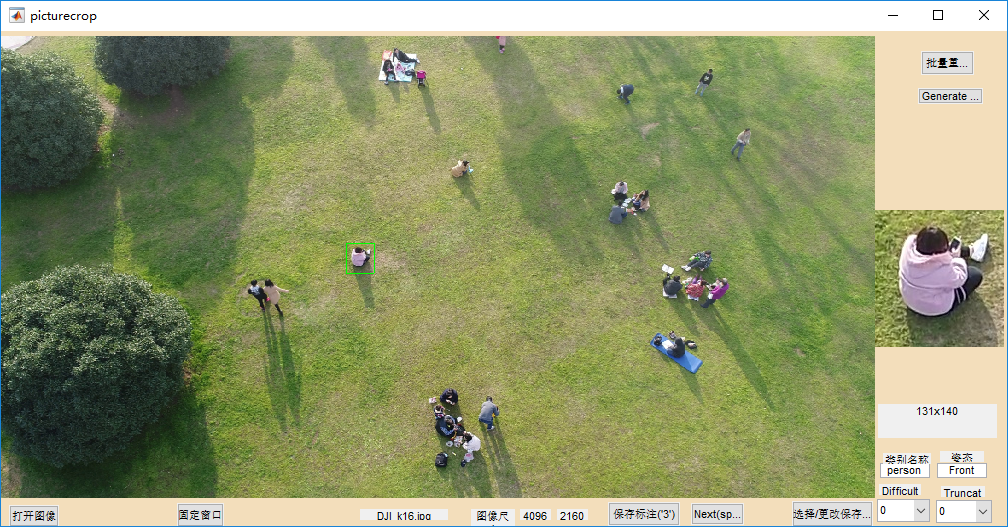
\includegraphics[height=7.62cm]{figures/数据集标注工具运行界面.png}
    \caption{数据集标注工具运行界面}\label{数据集标注工具运行界面}
\end{figure}

为了提高模型对视角变化的鲁棒性,主要使用的是斜视以及下视视野下的样本。经过标注之后,斜视85°,斜视45°以及下视的各种姿态下的人体训练图片数目比例大约为$1:1:1$。图\ref{标注样本示例}为标注的样本示例。

\begin{figure}[h]
    \centering
    \begin{subfigure}[h]{0.11\textwidth}
        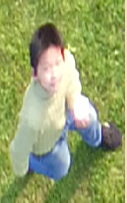
\includegraphics[width=\textwidth]{figures/样本标注示例1.png}
    \end{subfigure}
    ~ %add desired spacing between images, e. g. ~, \quad, \qquad, \hfill etc. 
      %(or a blank line to force the subfigure onto a new line)
    \begin{subfigure}[h]{0.11\textwidth}
        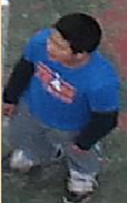
\includegraphics[width=\textwidth]{figures/样本标注示例2.png}
    \end{subfigure}
    ~ %add desired spacing between images, e. g. ~, \quad, \qquad, \hfill etc. 
    %(or a blank line to force the subfigure onto a new line)
    \begin{subfigure}[h]{0.11\textwidth}
        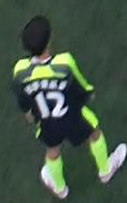
\includegraphics[width=\textwidth]{figures/样本标注示例3.png}
    \end{subfigure}
    \vskip1ex
    \begin{subfigure}[h]{0.11\textwidth}
        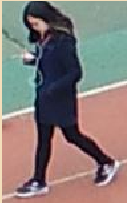
\includegraphics[width=\textwidth]{figures/样本标注示例4.png}
    \end{subfigure}
    ~ %add desired spacing between images, e. g. ~, \quad, \qquad, \hfill etc. 
      %(or a blank line to force the subfigure onto a new line)
    \begin{subfigure}[h]{0.11\textwidth}
        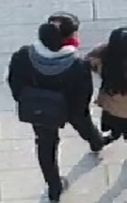
\includegraphics[width=\textwidth]{figures/样本标注示例5.png}
    \end{subfigure}
    ~ %add desired spacing between images, e. g. ~, \quad, \qquad, \hfill etc. 
    %(or a blank line to force the subfigure onto a new line)
    \begin{subfigure}[h]{0.11\textwidth}
        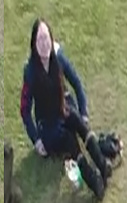
\includegraphics[width=\textwidth]{figures/样本标注示例6.png}
    \end{subfigure}
    \vskip1ex
        \begin{subfigure}[h]{0.11\textwidth}
        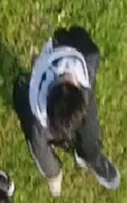
\includegraphics[width=\textwidth]{figures/样本标注示例7.png}
    \end{subfigure}
    ~ %add desired spacing between images, e. g. ~, \quad, \qquad, \hfill etc. 
      %(or a blank line to force the subfigure onto a new line)
    \begin{subfigure}[h]{0.11\textwidth}
        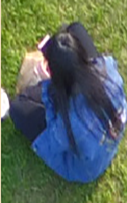
\includegraphics[width=\textwidth]{figures/样本标注示例8.png}
    \end{subfigure}
    ~ %add desired spacing between images, e. g. ~, \quad, \qquad, \hfill etc. 
    %(or a blank line to force the subfigure onto a new line)
    \begin{subfigure}[h]{0.11\textwidth}
        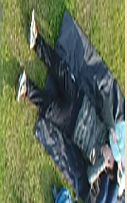
\includegraphics[width=\textwidth]{figures/样本标注示例9.png}
    \end{subfigure}
    \caption{标注样本示例。\\ 上:斜视85°;\quad 中:斜视45°;\quad 下:下视(斜视90°)}\label{标注样本示例}
\end{figure}

对于训练,本论文使用的机器配置如下:CPU为32核心i7-6700K,GPU为4路8GB内存的GTX1080显卡,内存为128GB。

将原始SSD算法的基础网络更改为残差网络,针对自建数据集训练模型参数,得到修改后的SSD目标检测模型。
SSD实际目标检测结果如图\ref{改进SSD无人机视角目标检测结果}所示。
 	 
\begin{figure}[h]
    \centering
    \begin{subfigure}[h]{0.42\textwidth}
        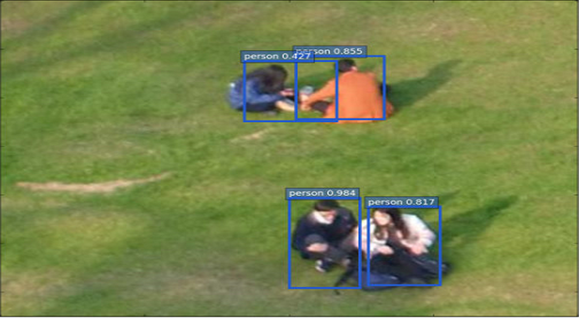
\includegraphics[width=\textwidth]{figures/改进SSD无人机视角目标检测结果1.png}    
    \end{subfigure}
    ~
    \begin{subfigure}[h]{0.42\textwidth}  
        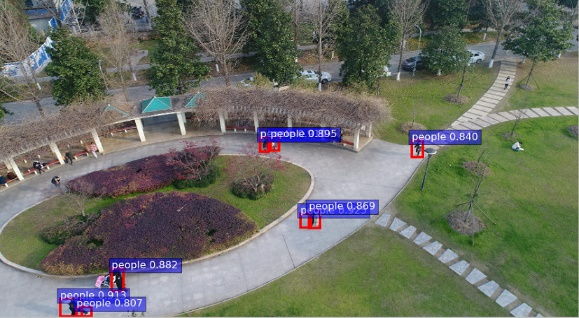
\includegraphics[width=\textwidth]{figures/改进SSD无人机视角目标检测结果2.jpg}   
    \end{subfigure}
    \vskip1ex
    \begin{subfigure}[h]{0.42\textwidth}   
        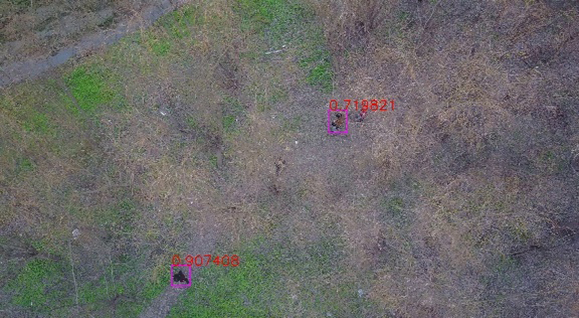
\includegraphics[width=\textwidth]{figures/改进SSD无人机视角目标检测结果3.jpg}  
    \end{subfigure}
    ~
    \begin{subfigure}[h]{0.42\textwidth}
        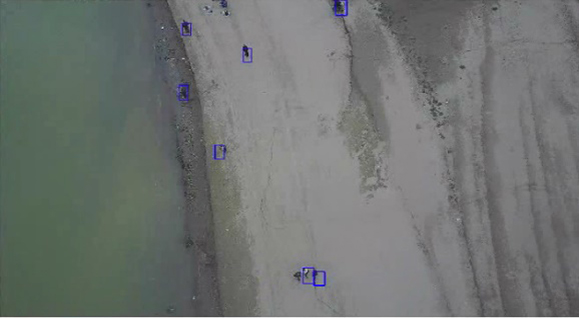
\includegraphics[width=\textwidth]{figures/改进SSD无人机视角目标检测结果4.jpg}   
    \end{subfigure}

    \caption{改进SSD无人机视角目标检测结果}\label{改进SSD无人机视角目标检测结果}
\end{figure}


平均耗时:0.06s/每张图。

由实验结果即图\ref{改进SSD无人机视角目标检测结果}可以看出,改进后的SSD算法对于各种姿态以及视角,如蹲坐(左上),斜视(右上),下视以及遮挡(左下)都有着较好的检测效果。

同时,我们还进行了一系列的对比实验,对比了传统目标检测算法DPM、基于深度学习的检测算法Faster-RCNN、改进前的SSD算法以及改进后的SSD算法在本数据集上的检测性能。实验对比了四种算法的P-R曲线图,检测结果如图\ref{PR}所示。
\begin{figure}[h]
    \centering
    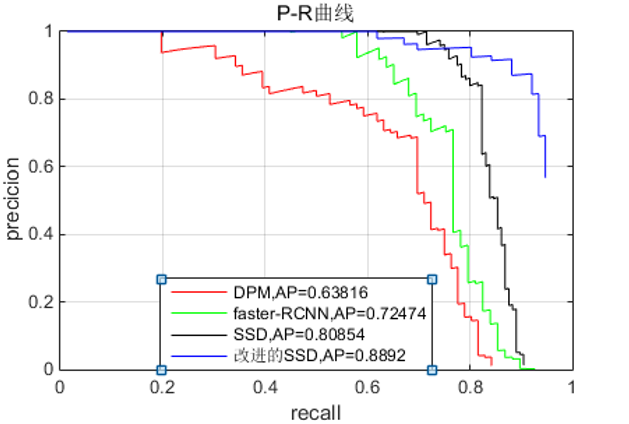
\includegraphics[height=7cm]{figures/PR曲线.png}
    \caption{四种流行的检测算法的P-R曲线图}\label{PR}
\end{figure}

从图\ref{PR}中可以看出,在本数据集上,改进后的SSD算法表现最优,平均检测精度AP达到0.8892。


\section{自主避障实验结果}

对于第四章中介绍的基于双目视觉的自主避障技术,在实际环境中进行了多次实验。由于实验场地的限制,测试的场景比较有限,主要测试了无人机系统对于墙壁、树木等静止障碍的躲避,以及移动障碍(行人)的躲避。

本部分,根据无人机实际尺寸设置一个“膨胀系数”以及“安全距离”,分别用于设置实际避障使用到的无人机尺寸以及距离障碍物的最小距离,实验中,M100对角线(包含保护罩)的长度为$1m$,因此设置膨胀系数为$1.2$,安全距离为$0.5m$,这样,实际上当无人机旋翼末端距离障碍$70cm$的时候为极限距离。实际飞行试验中,设置无人机前进方向的最大飞行速度为$2m/s$进行实验。

实际障碍点云图以及规划的避障路线如图\ref{3D}所示。规划的避障路线是根据障碍物信息不断更新的。
\begin{figure}[h]
    \centering
    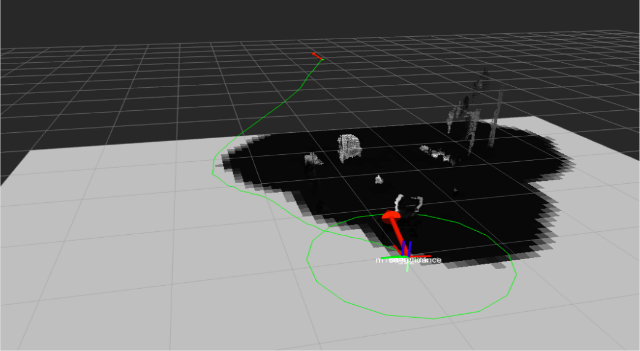
\includegraphics[height=4.05cm]{figures/双目视觉生成的3D障碍点云以及规划的避障路径.png}
    \caption{双目视觉生成的3D障碍点云以及规划的避障路径}\label{3D}
\end{figure}

实际自主避障实验结果如图\ref{Avoid}。
 	 
\begin{figure}[h]
    \centering
    \begin{subfigure}[h]{0.475\textwidth}
        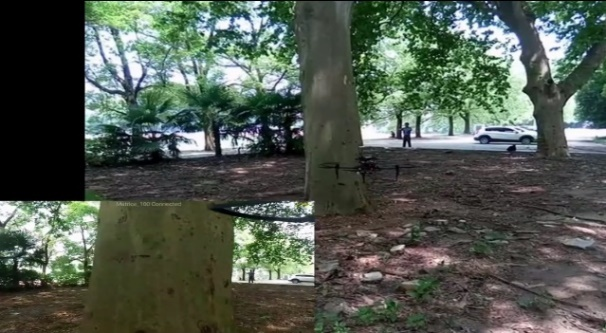
\includegraphics[width=\textwidth]{figures/自主避障1.jpg}    
    \end{subfigure}
    ~
    \begin{subfigure}[h]{0.475\textwidth}  
        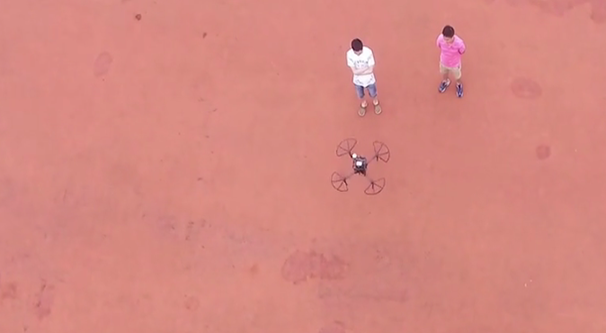
\includegraphics[width=\textwidth]{figures/自主避障2.png}   
    \end{subfigure}
    \vskip1ex
    \begin{subfigure}[h]{0.475\textwidth}   
        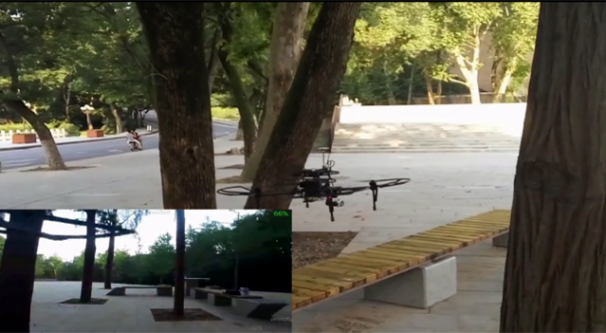
\includegraphics[width=\textwidth]{figures/自主避障3.png}  
    \end{subfigure}
    ~
    \begin{subfigure}[h]{0.475\textwidth}    
        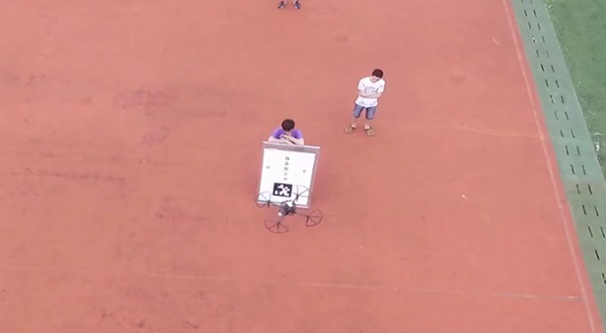
\includegraphics[width=\textwidth]{figures/自主避障4.jpg}   
    \end{subfigure}

    \caption{躲避树木; 躲避行人}\label{Avoid}
\end{figure}

经过测试,发现系统不仅对墙壁这种简单的平面障碍躲避灵敏,还可以在错落复杂的大树之间穿梭以及躲避移动的障碍(行人)。因此有理由相信,对于实际野外搜救中可能遇到的电线杆,铁塔等高大建筑,也可以达到较好的效果,限于实验环境,尚未进行相应的试验。


\section{移动降落实验结果}

对于无人机移动降落实验,设置如下的试验方案。

打印A0大小的系列AprilTag标志,标志如下排列。采用大小标志组合主要基于两个考虑:

1. 无人机高空快速锁定降落点

无人机在空中飞行时($10\sim20m$),地面标志成像大小需要足够大以完成标志检测识别,此时只需检测大尺寸标志。

2. 垂直降落过程中,接近降落平面时,无人机光学相机无法获取大标志的全貌,因此改为检测小标志,做进一步的姿态调整,从而实现精准降落。

实验中,将打印的标志图案贴于长宽分别为:$1.7m,1.2m$的白板上,大小模拟普通敞篷皮卡后备车厢大小。分别放置在武汉大学工学部风雨操场上不同位置,设置无人机根据GPS(位置精度$5m$)飞行至标志上方,然后系统自行检测降落标志,根据解算得到的相机姿态,飞行到标志正上方,为了保证在靠近过程中标志始终不移出无人机视野,系统对相机的姿态进行动态调整,使得标志始终处于视野中心。

\begin{figure}[h]
    \centering
    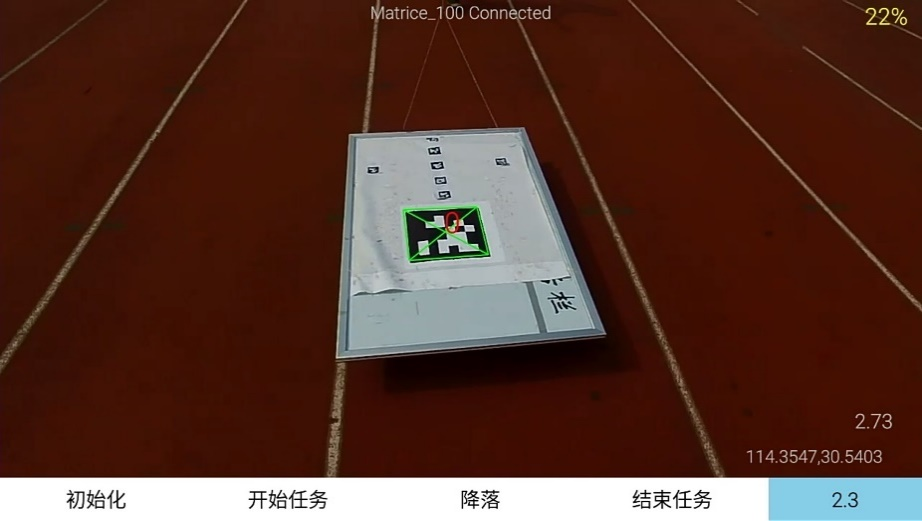
\includegraphics[width=12cm]{figures/移动降落.jpg}
    \caption{降落标志保持在视野中心(无人机相机视角视图)}\label{Landing}
\end{figure}


当无人机飞行至标志正上方之后,固定相机为$90^\circ$朝下,以$0.5m/s$的速度垂直下降,下降到距离降落平面$1.3m$之后切换为检测小标志(主要是与大标志共线的小标志,取平均值)并做最后的降落引导。

进行20次实验,以降落平面中心为基准点,测得降落点(飞机质心投影)距离其的位置偏差标准差为:
X方向:$+11cm$,Y方向:$+9cm$。
此降落精度下,该20次试验,无人机均成功落在白板上,没有超出界限,如图\ref{Landing}左图。

\begin{figure}[h]
    \centering
    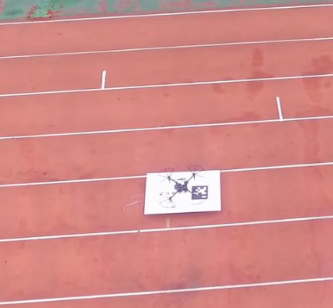
\includegraphics[height=4cm]{figures/移动降落卡车1.png}
    \quad
    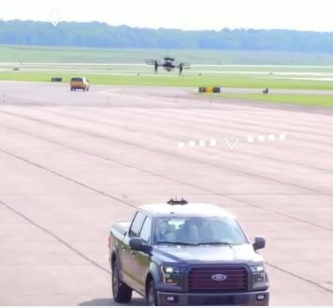
\includegraphics[height=4cm]{figures/移动降落卡车2.png}
    \caption{ 降落在平板上(左); 降落在皮卡后部(右)}\label{Landing}
\end{figure}

此外,本系统进行了一次成功的降落在真实皮卡上的实验,证明了本系统移动降落的可行性。 


\section{配套演示系统}

由于本系统是多模块集成系统,飞机端的数据处理以及指令传输主要是在机器人操作系统ROS上进行,无需图形化界面。对于地面站端,出于实际需求考虑,本系统包含一个配套的演示系统。其中包括一个移动端App,负责以下功能:
\begin{enumerate}[1.]
\item 充当机载计算设备与地面计算设备的中介。通过建立移动设备和无线笔记本的TCP通信链路,由此地面计算设备(笔记本电脑)将能够获取到飞行端回传的候选区域系列坐标,以便进行下一步的光学检测。
\item 提供必要的交互,包括系统初始化,设定起始搜索点(GPS坐标),拍照,录像以及返航等功能。
\item 飞行器状态信息显示,主要是一些重要的飞行器状态信息,如电池剩余量,飞行高度,实时GPS等信息等。
\end{enumerate}

移动端APP运行界面如图\ref{配套移动应用运行界面}所示。

\begin{figure}[h]
    \centering
    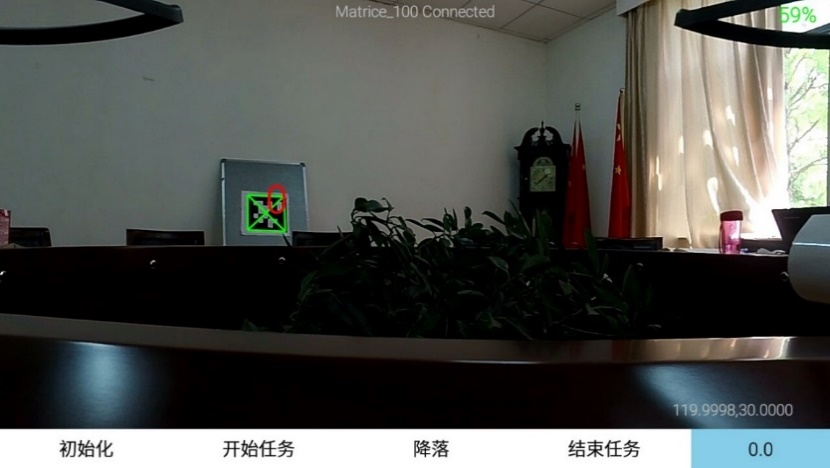
\includegraphics[width=12cm]{figures/配套移动应用运行界面.jpg}
    \caption{配套移动应用运行界面}\label{配套移动应用运行界面}
\end{figure}

系统运行时,首先点击初始化,获取无人机的控制权,然后输入起始搜索点的经纬度坐标。点击开始任务,则无人机开始起飞,飞向指定搜索起始点,并以之字形扫描搜索区域。飞行过程中无人机进行红外图像处理以及自主避障,直到搜索检测到目标之后,悬停,等待地面的指令:是否继续搜索。点击结束任务,则无人机返回起飞点上方,并启动自动移动降落程序,准确着陆在降落平台上。

为了方便地面工作人员观察评判目标检测结果,在地面笔记本电脑上开发了一个GUI界面程序。程序采用Qt5跨平台工具,在Linux系统上进行开发。采用多线程编程,将UI和图像处理分开处理,使得处理结果显示流畅。由于预先得到了候选区域(红外检测给出),实际应用于光学检测时,1080P分辨率的图片可以达到22FPS的处理速度,基本达到实时。

\begin{figure}[h]
    \centering
    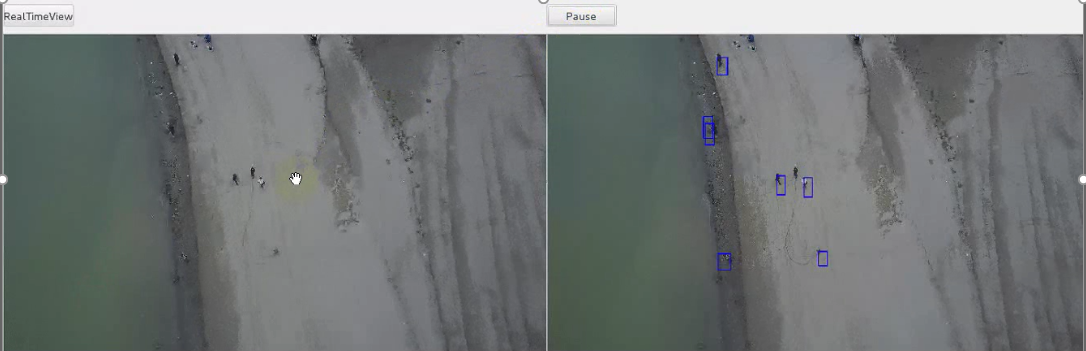
\includegraphics[height=5cm]{figures/光学处理GUI程序运行界面.png}
    \caption{光学处理GUI程序运行界面}\label{光学处理GUI程序运行界面}
\end{figure}

图\ref{光学处理GUI程序运行界面}是PC端软件运行界面,左边为实时预览界面,右边是检测结果,均支持局部放大和拖动。点击"开始"按钮就可进行光学检测。检测结果将使用蓝色包围框框住。下方显示目标当前所在GPS经纬度。

经过实际测试,本系统各功能运行正常,各模块响应速度快,飞行试验30余次均未出现故障。
